\section{Resultados Numéricos}

\begin{frame}
    \frametitle{\secname}

    Vamos a realizar experimentos que ratifican algunos resultados vistos en la teoría.
    Estos experimentos van a ser aplicados a la ecuación de transporte
    dada por

    \begin{equation}\label{eq:transportequation}
        u_{t}
        \left(x,t\right)+
        cu_{x}
        \left(x,t\right)=
        0,\quad
        x\in\mathbb{R},\quad
        t>0,
    \end{equation}

    siendo $c$ es la velocidad de propagación.

    \begin{example}
        En este ejemplo consideramos el dominio espacial
        $\Omega=\left[0,20\right]$, el paso en espacio $\Delta x=0.1$, el
        paso en tiempo $\Delta t=0.02$, la velocidad de propagación negativa
        $c=-1$ (para los que se verifica la condición CFL) y la condición
        inicial dada por

        \begin{equation*}
            u_{0}=
            e^{-{\left(x-15\right)}^{2}}.
        \end{equation*}

        Para estos datos calculamos las soluciones numéricas de la ecuación
        de transporte~\eqref{eq:transportequation} con condición inicial,
        aplicando el método descentrado downwind, el método de Lax-Friedrichs
        y por último, el método de Lax-Wendroff.
        Para ello, hemos empleado el lenguaje de programación Python.
        Así, obtenemos los resultados de las Figuras~\ref{fig:example1t2}
        y~\ref{fig:example1t40}, para cada uno de los métodos estudiados
        junto con la solución exacta para cada instante de tiempo
        considerado.
    \end{example}
\end{frame}

\begin{frame}
    \frametitle{\secname}
    \begin{figure}[ht!]
        \centering
        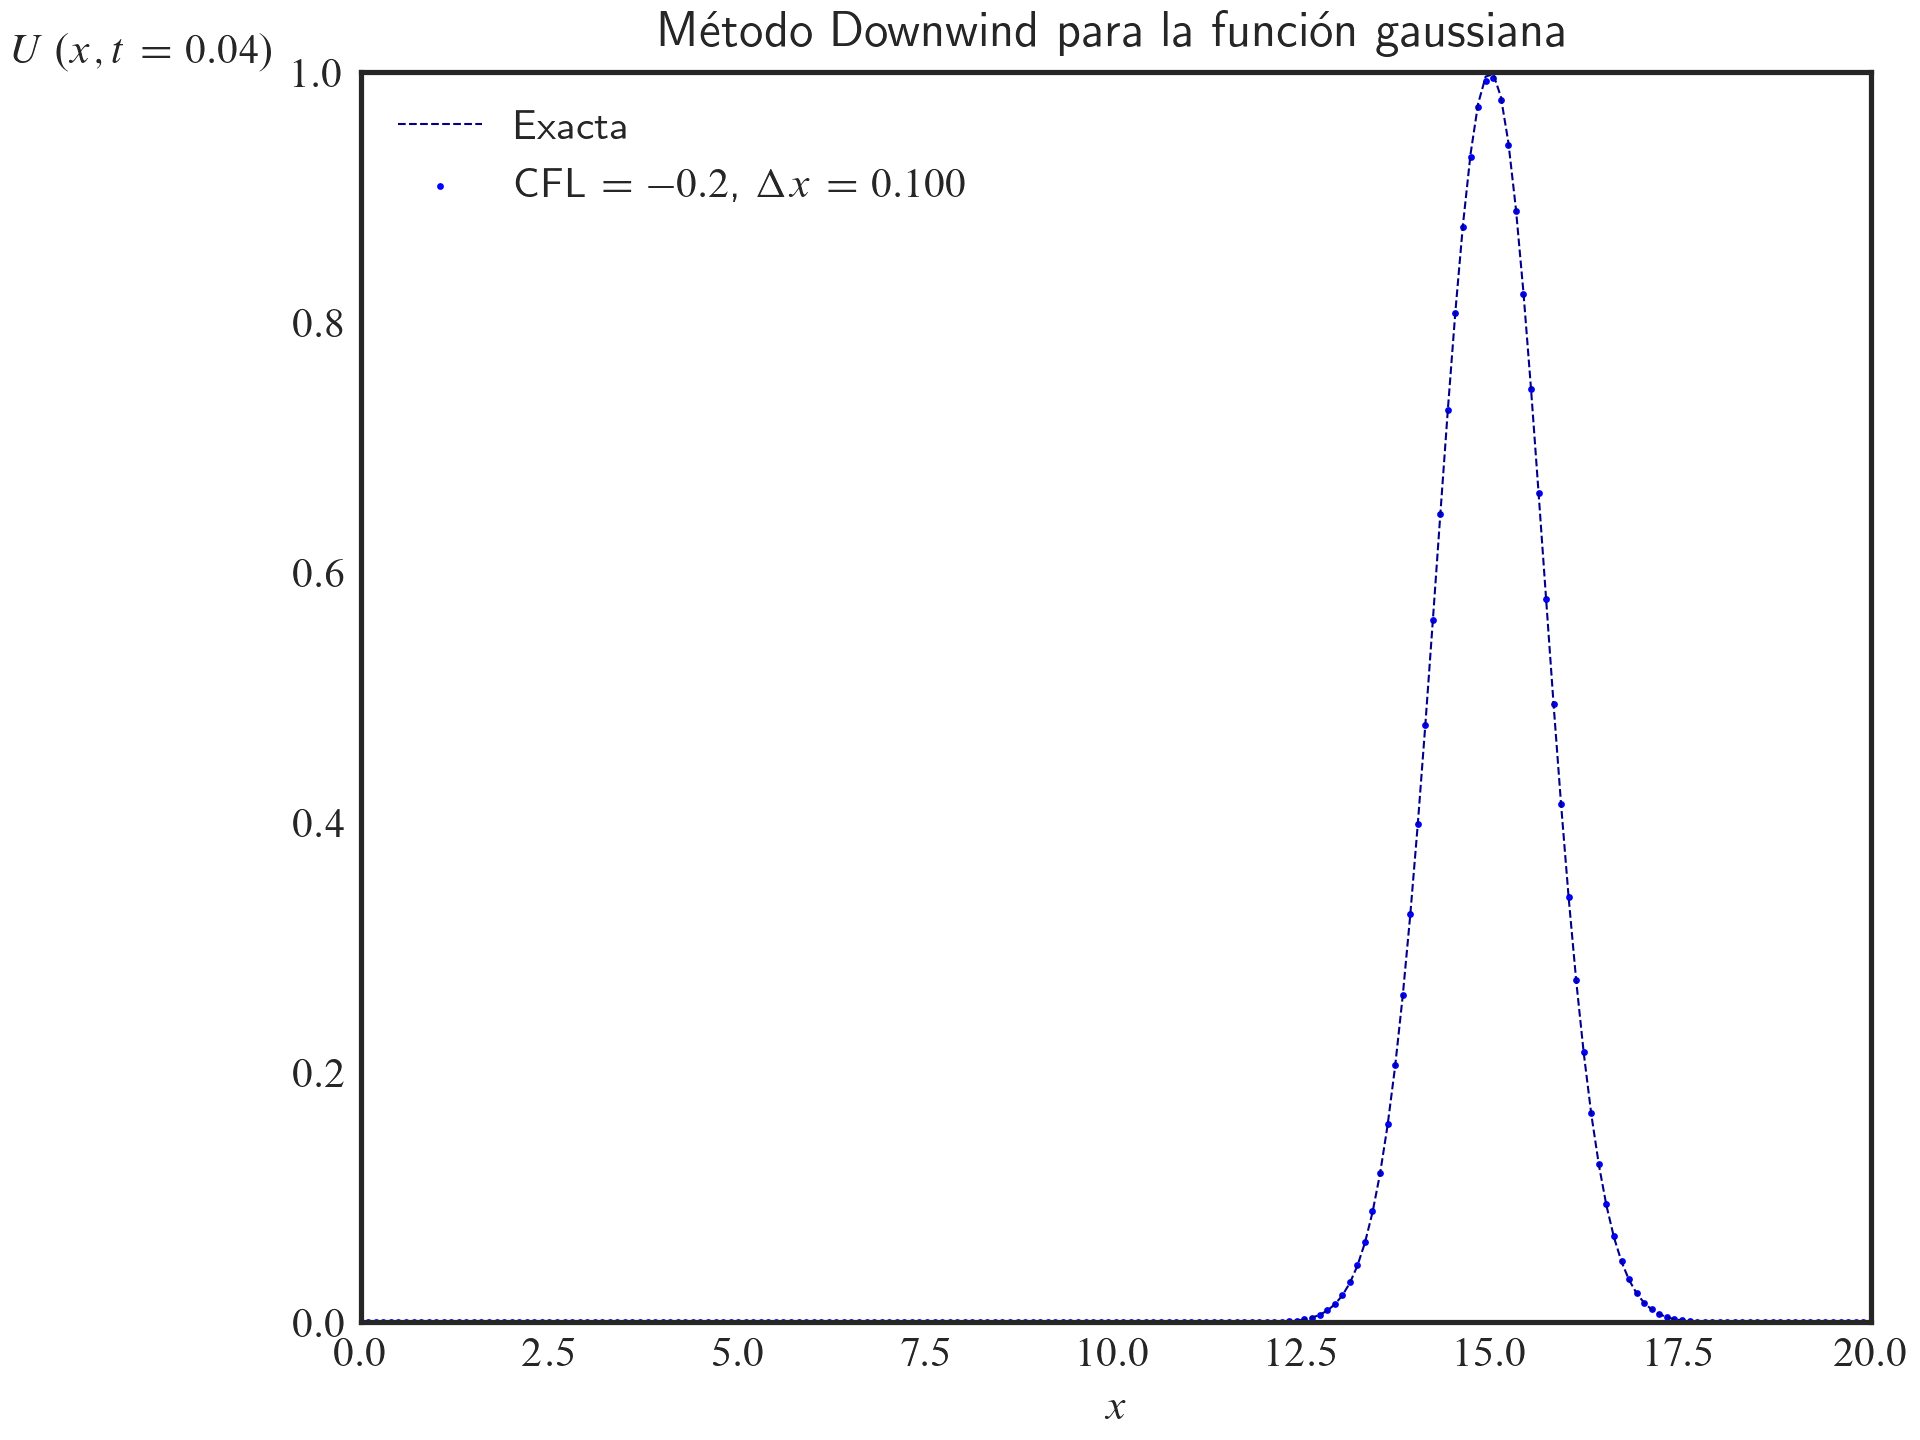
\includegraphics[width=.30\paperwidth]{../snapshots/downwindgaussian1d-2.png}
        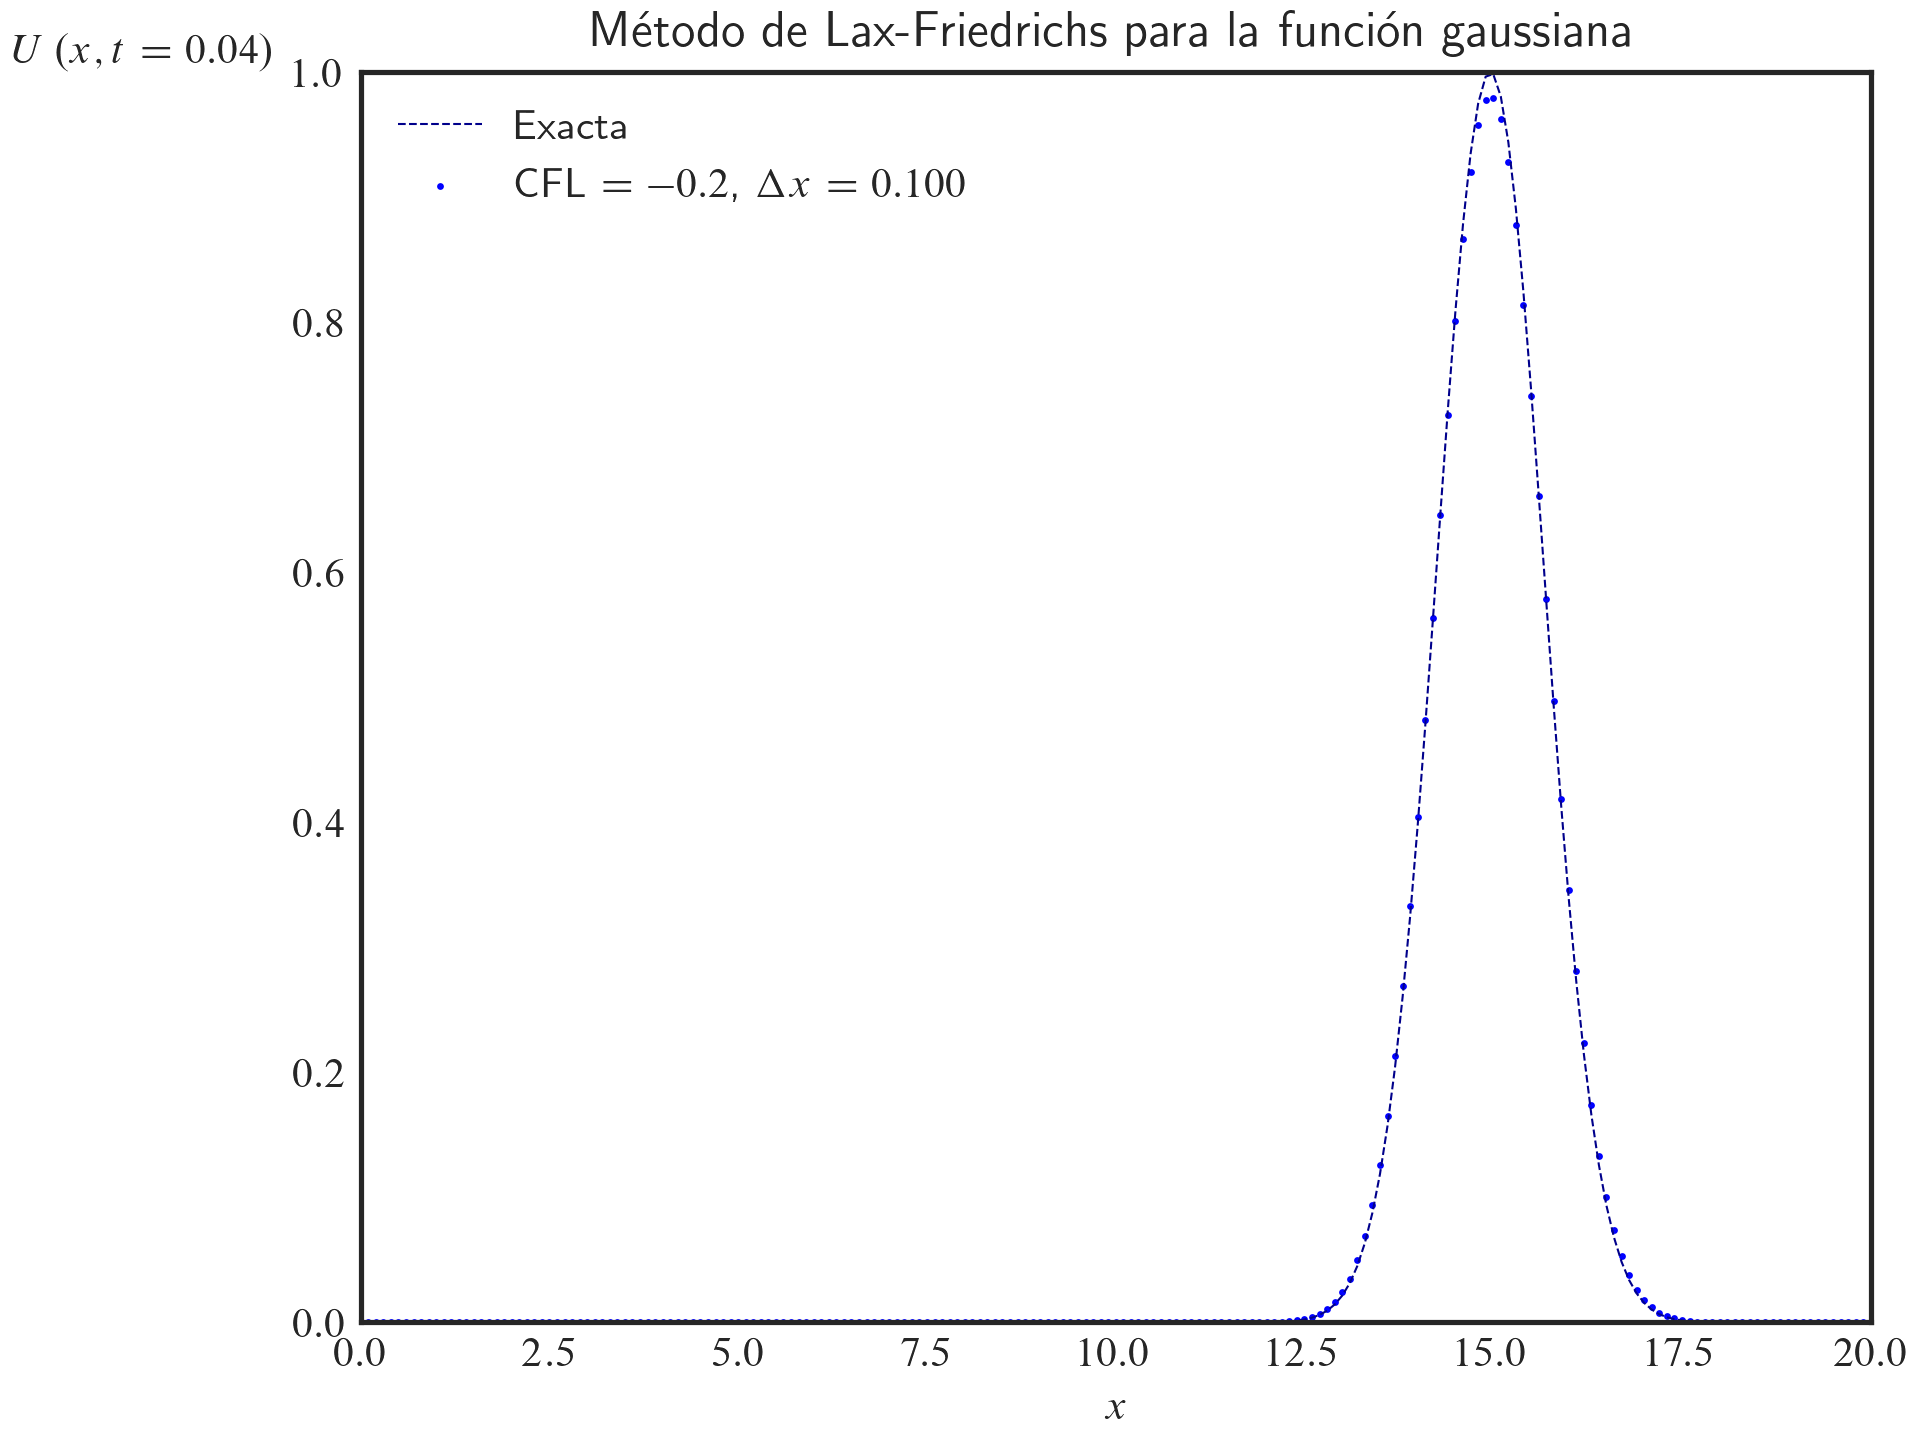
\includegraphics[width=.30\paperwidth]{../snapshots/lax-friedrichsgaussiana1d-2.png}
        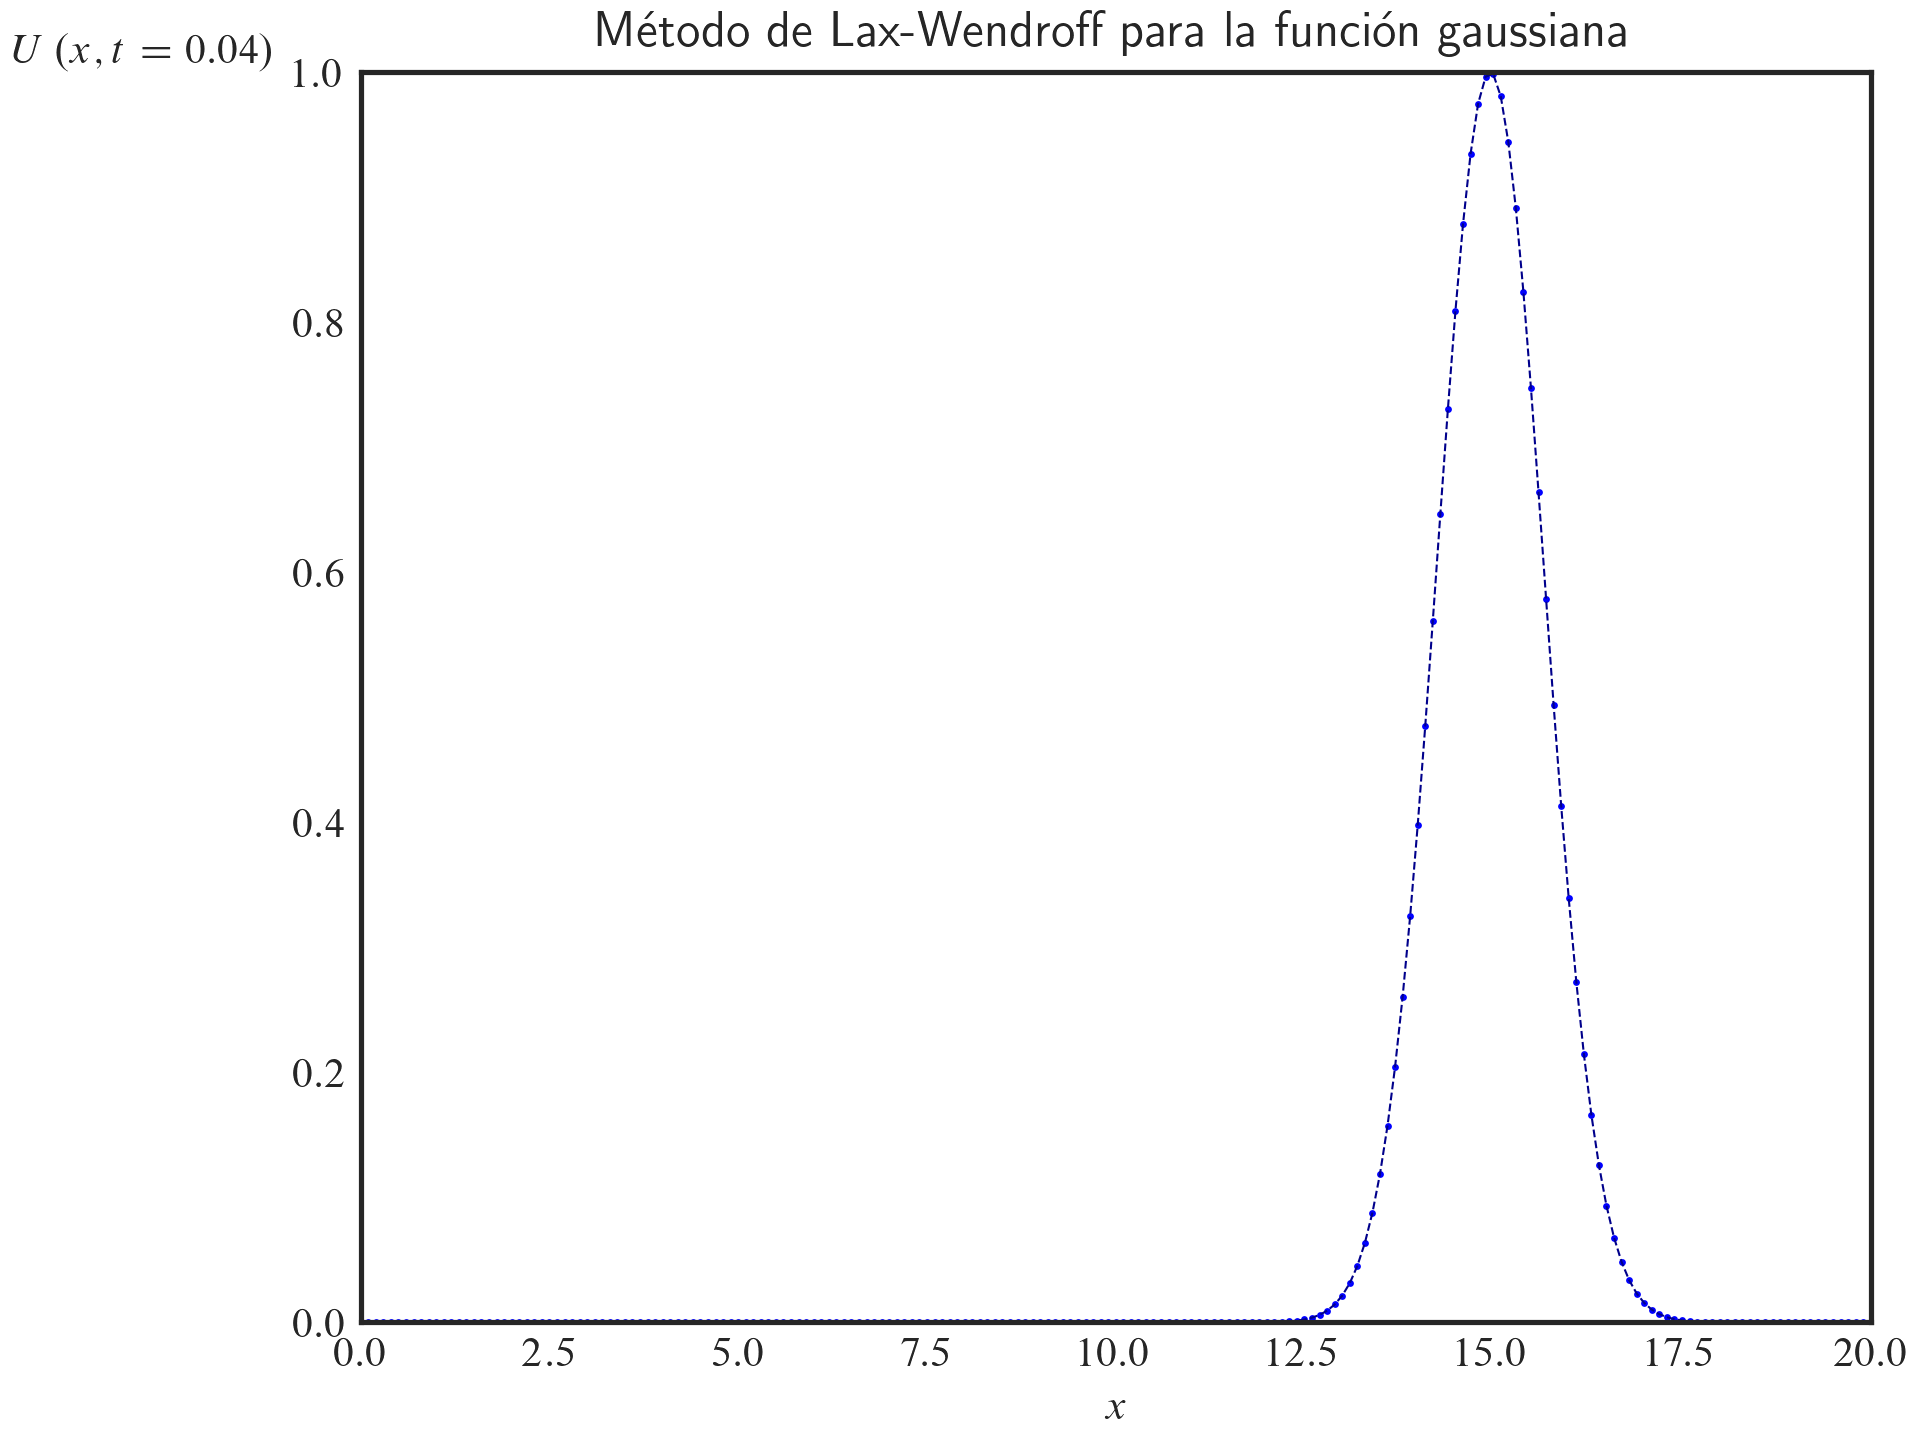
\includegraphics[width=.30\paperwidth]{../snapshots/lax-wendroffgaussiana1d-2.png}
        \caption{Simulación numérica en el tiempo $t_{2}=2\Delta t$.}
        \label{fig:example1t2}
    \end{figure}
\end{frame}

\begin{frame}
    \frametitle{\secname}

    \begin{figure}[ht!]
        \centering
        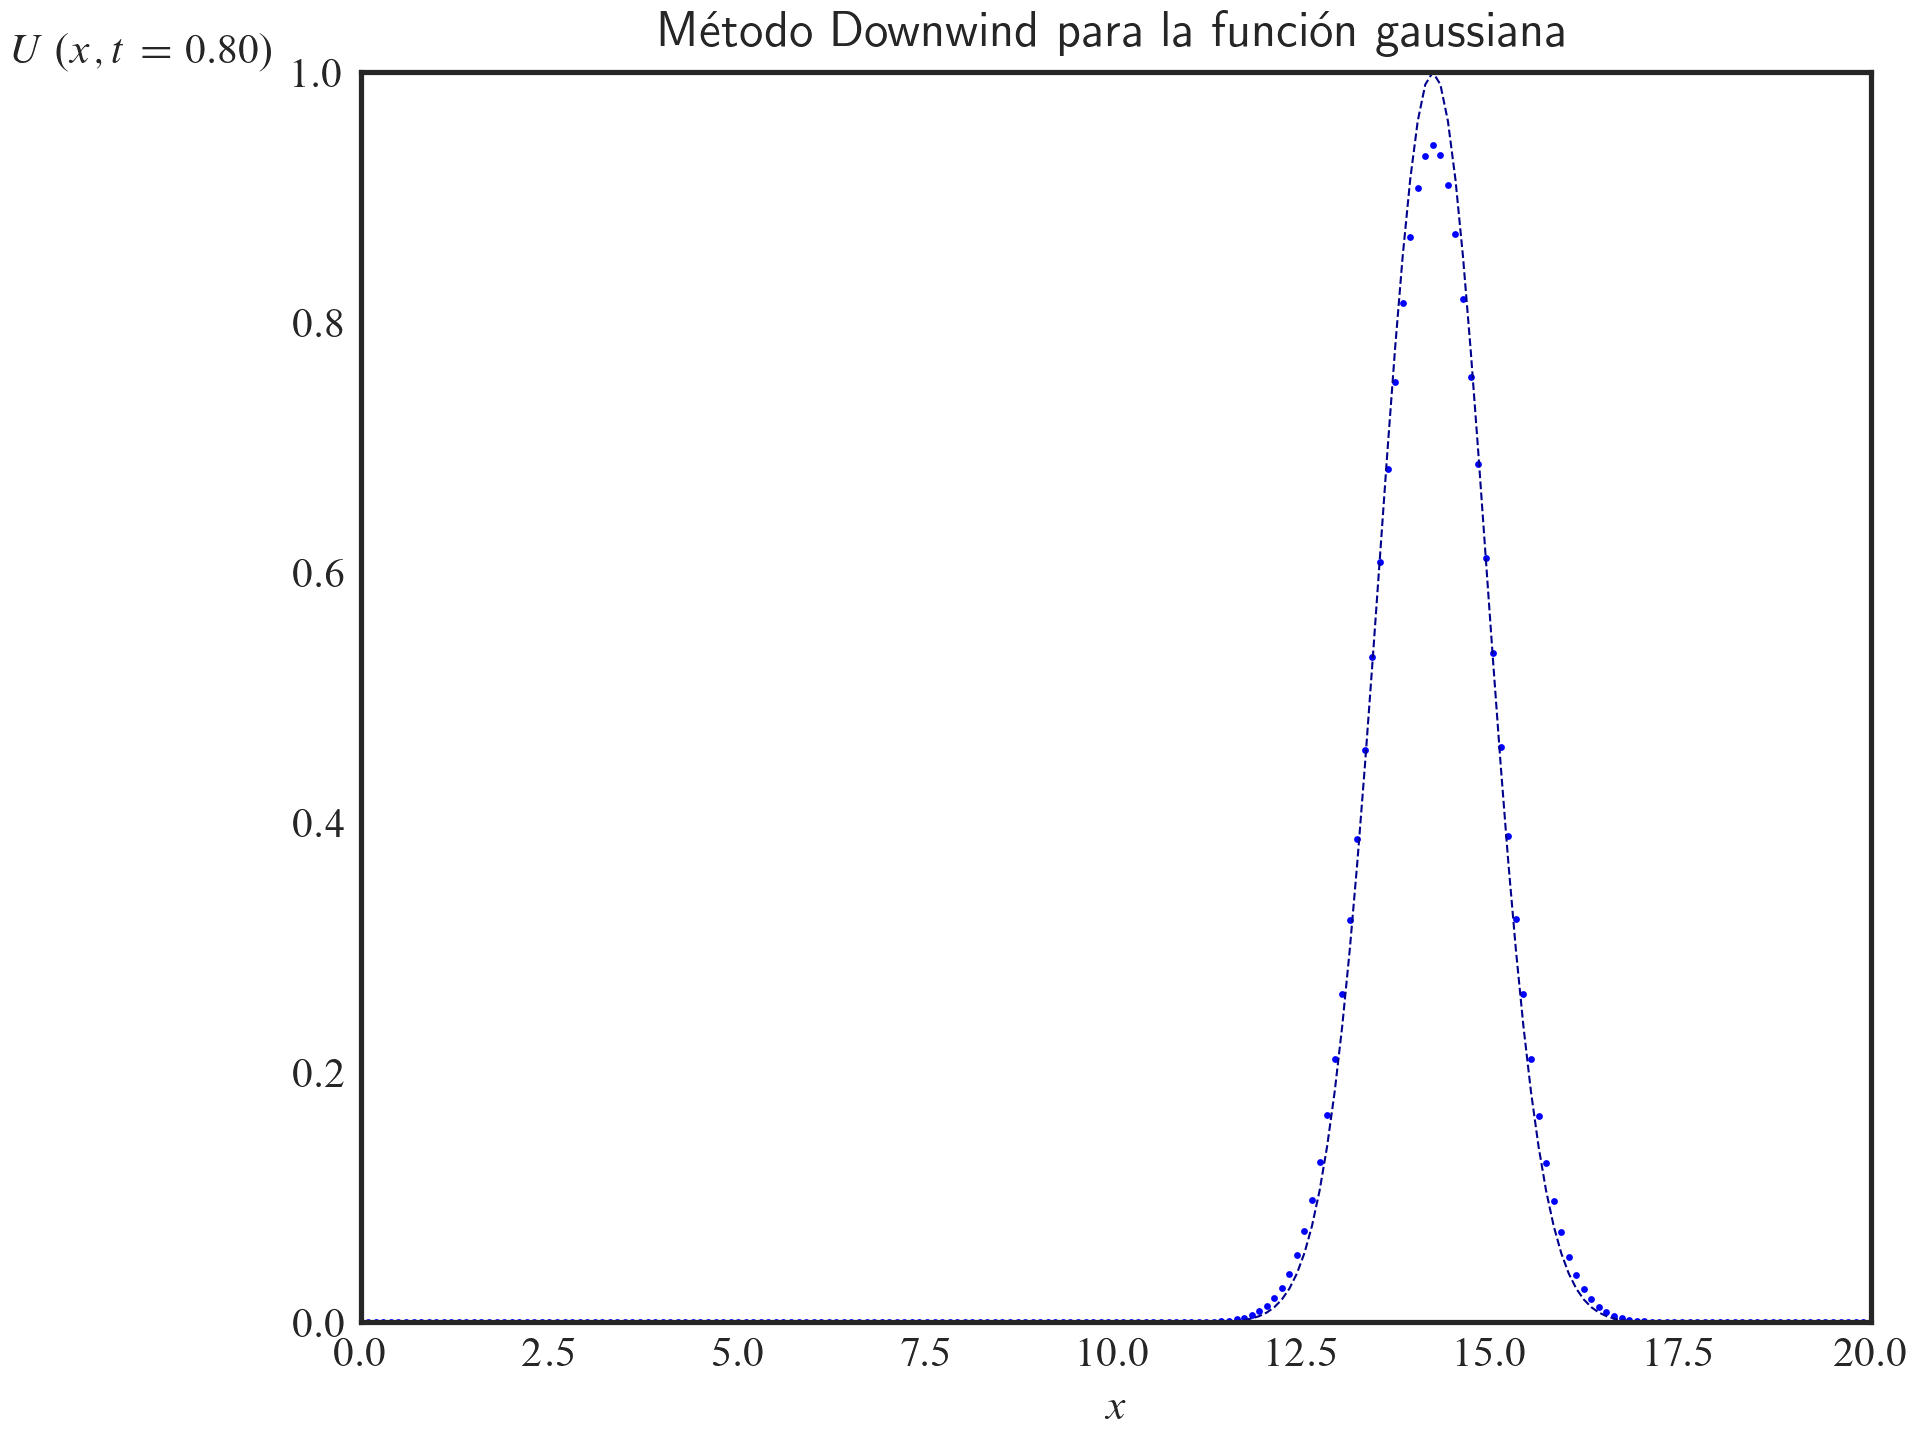
\includegraphics[width=.30\paperwidth]{../snapshots/downwindgaussian1d-40.png}
        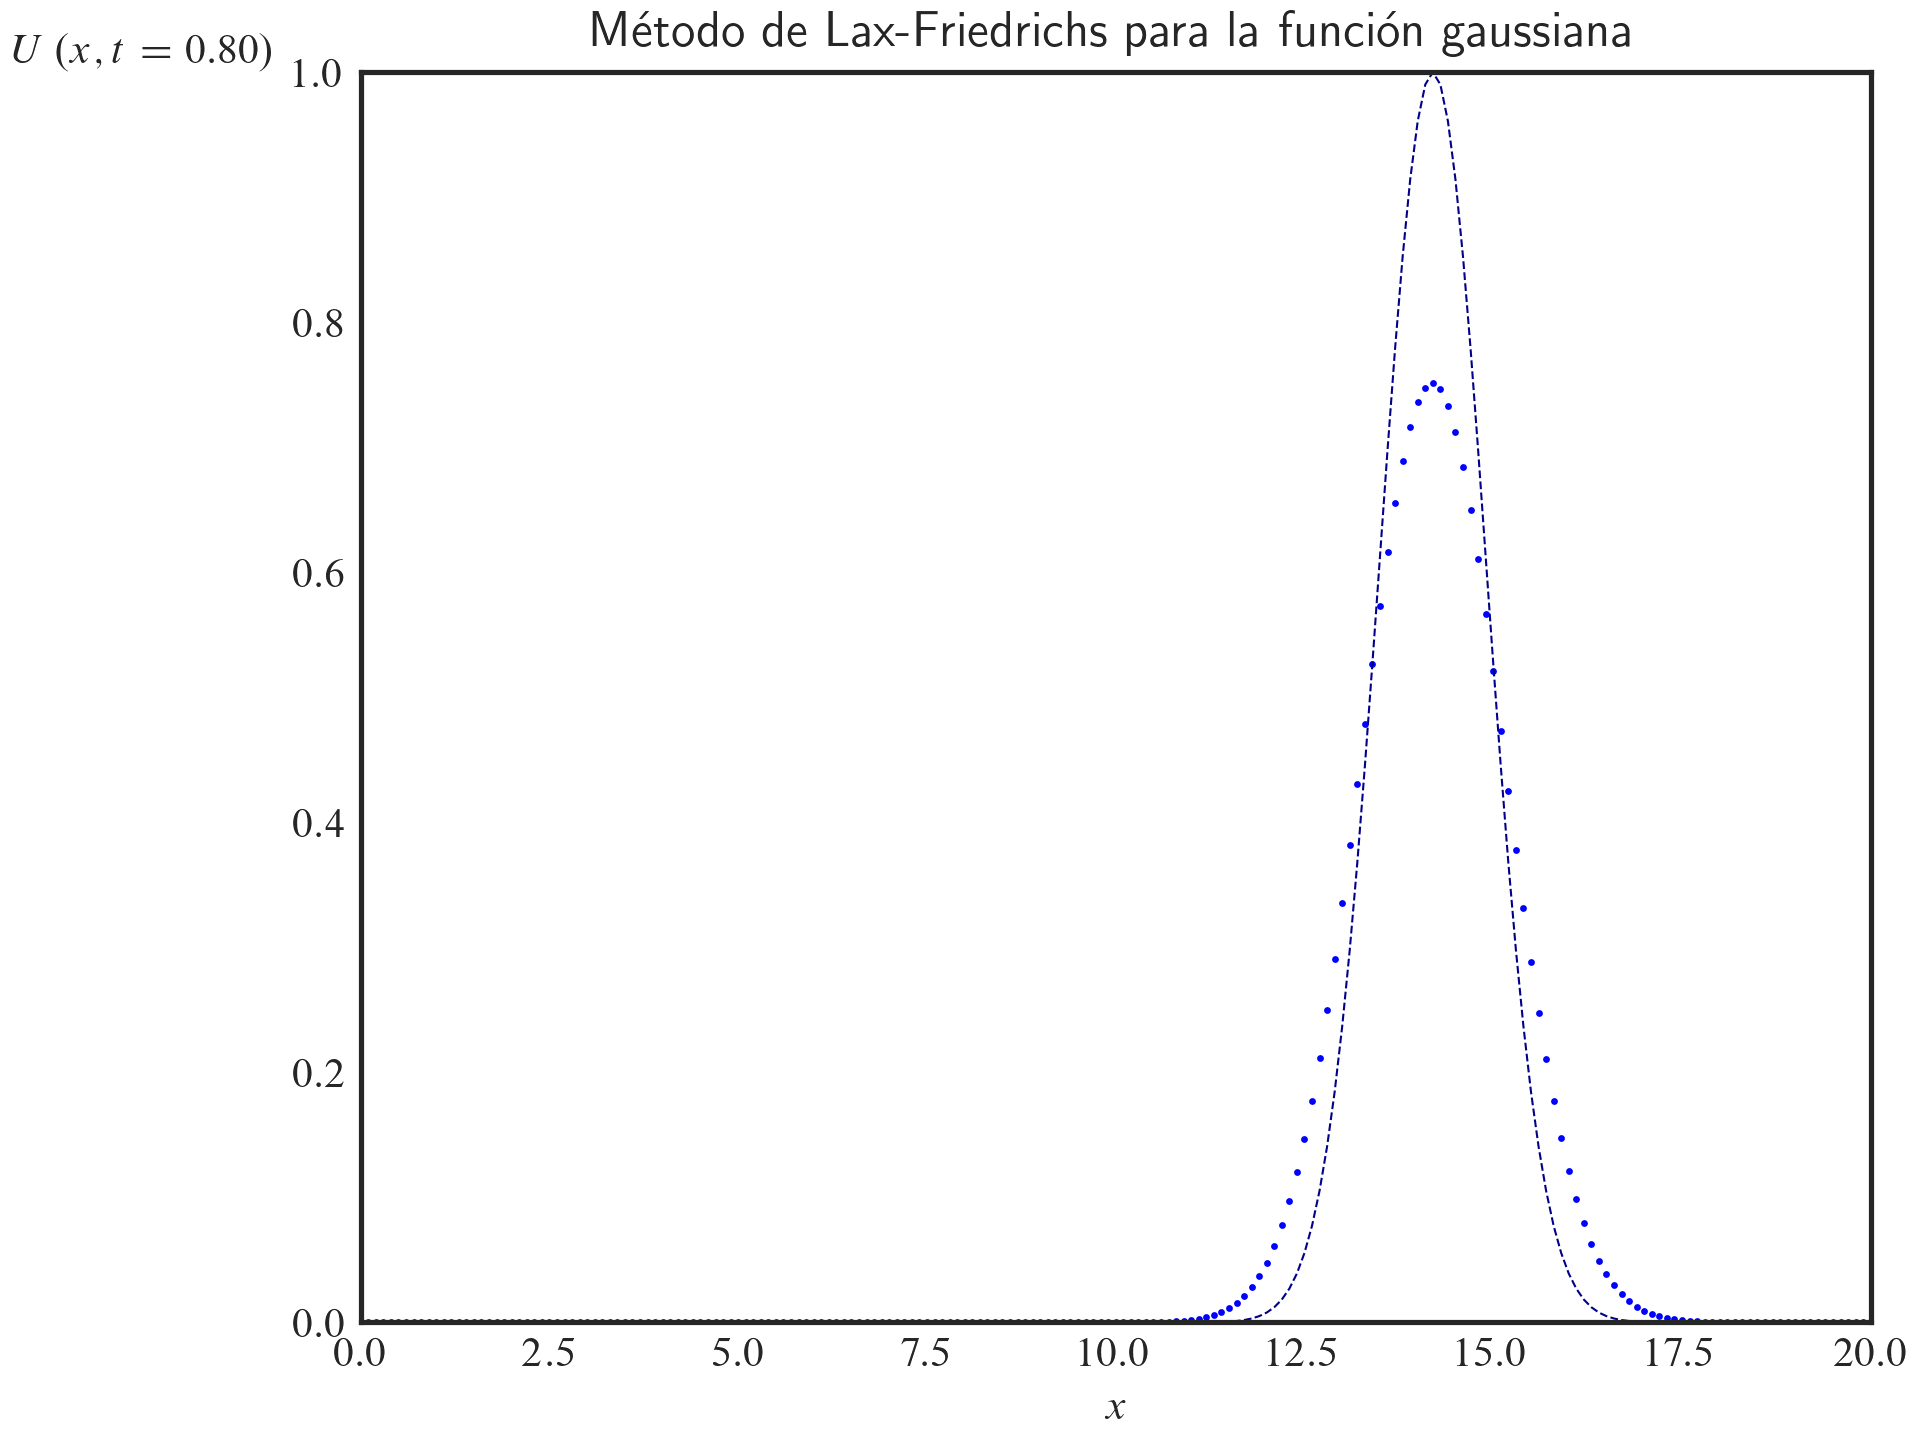
\includegraphics[width=.30\paperwidth]{../snapshots/lax-friedrichsgaussiana1d-40.png}
        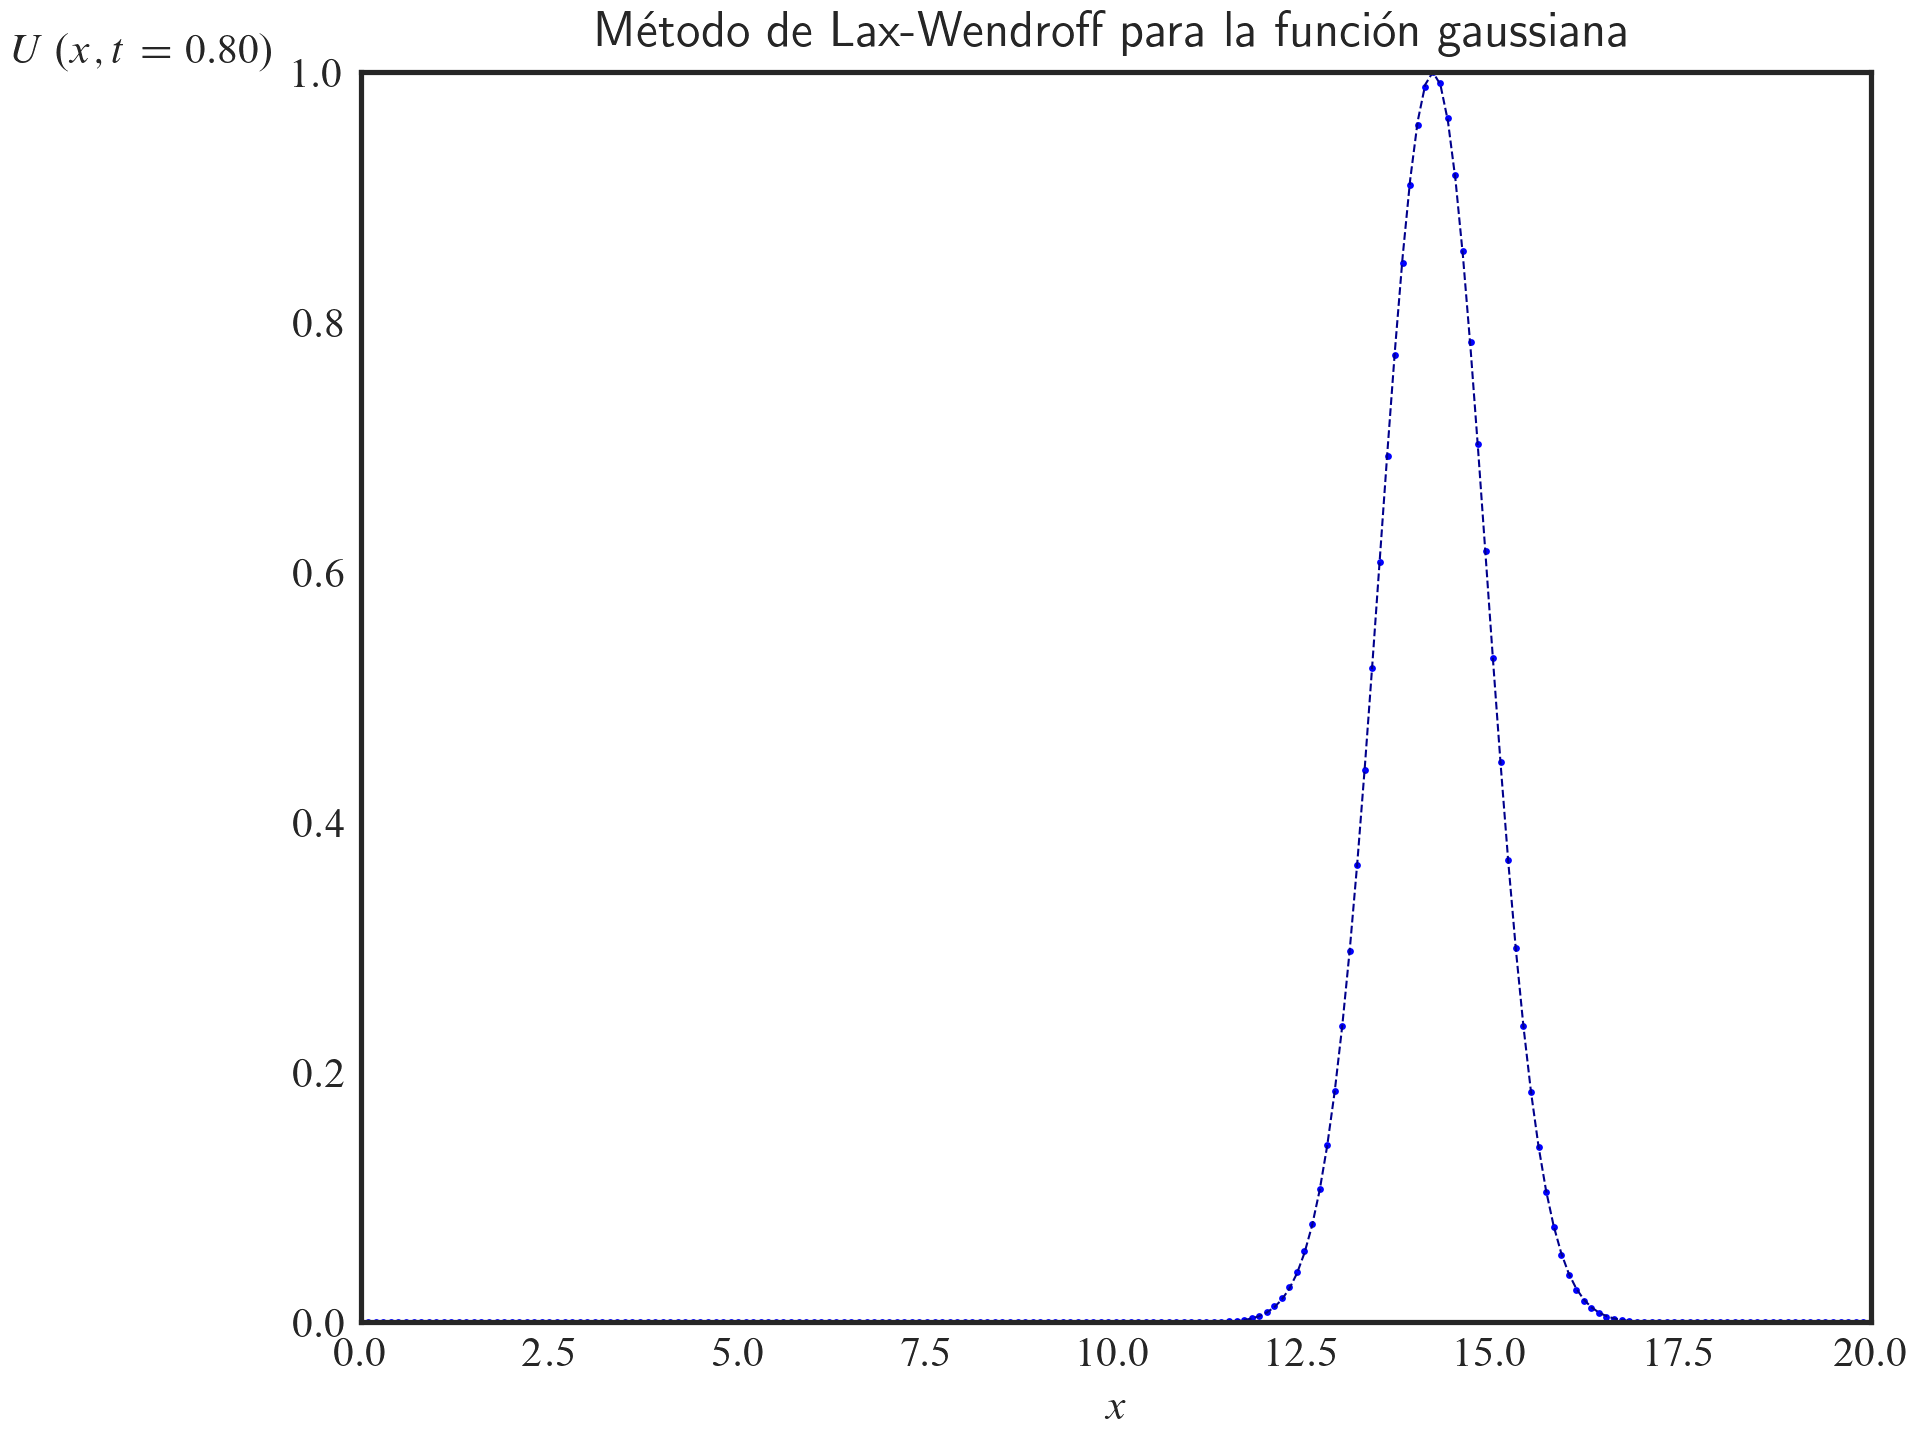
\includegraphics[width=.30\paperwidth]{../snapshots/lax-wendroffgaussiana1d-40.png}
        \caption{Simulación numérica en el tiempo $t_{40}=40\Delta t$.}
        \label{fig:example1t40}
    \end{figure}
\end{frame}

\begin{frame}
    \frametitle{\secname}
    \begin{example}
        En este ejemplo consideramos el dominio espacial
        $\Omega=\left[0,30\right]$, el paso en espacio $\Delta x=0.12$, el
        paso en tiempo $\Delta t=0.02$, la velocidad de propagación positiva
        $c=1$ (para los que se verifica la condición CFL) y la condición
        inicial dada por la función discontinua

        \begin{equation*}
            u_{0}\left(x\right)=
            \begin{cases}
                2, & \text{si }x<15, \\
                1, & \text{si }x>15.
            \end{cases}
        \end{equation*}

        Para este dato inicial calculamos las soluciones numéricas de la
        ecuación de transporte~\eqref{eq:transportequation}, aplicando el
        método descentrado upwind, el método de Lax-Friedrichs y por último,
        el método de Lax-Wendroff.
        Al igual que en el ejemplo anterior, hemos empleado el lenguaje de
        programación Python.
        Entonces, obtenemos los resultados de las
        Figuras~\ref{fig:example2t2} y~\ref{fig:example2t10} (donde se
        reproduce el mismo experimento pero en los instantes de tiempo
        $t_{2}=0.04$ y $t_{10}=0.2$), para cada uno de los métodos nombrados
        junto con la solución exacta y para cada instante de tiempo
        considerado.
    \end{example}
\end{frame}

\begin{frame}
    \frametitle{\secname}

    \begin{figure}[ht!]
        \centering
        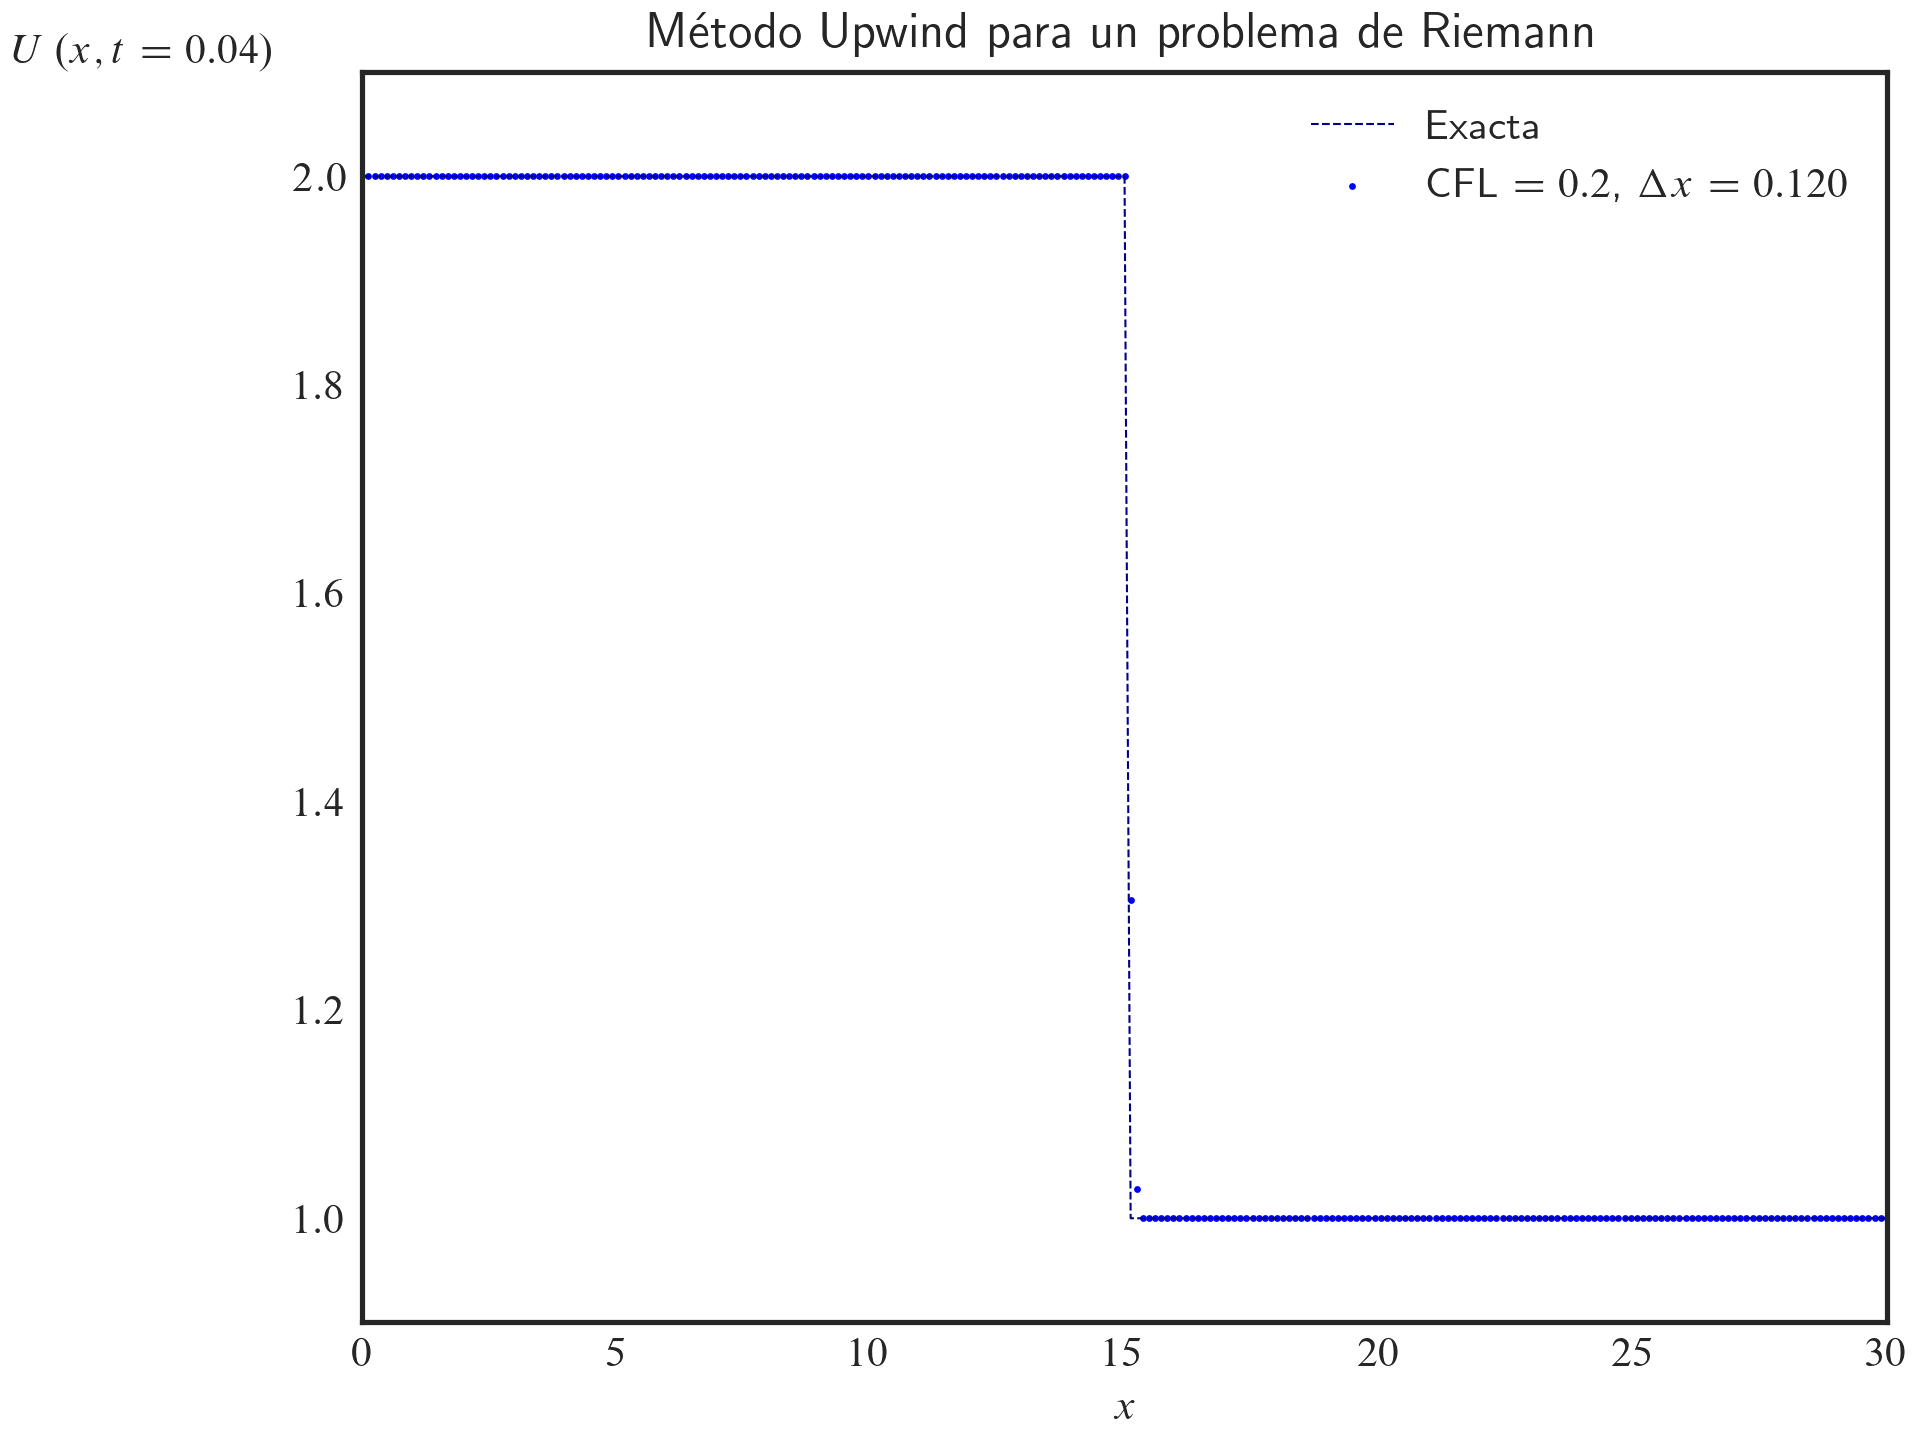
\includegraphics[width=.30\paperwidth]{../snapshots/upwindheaviside1d-2.png}
        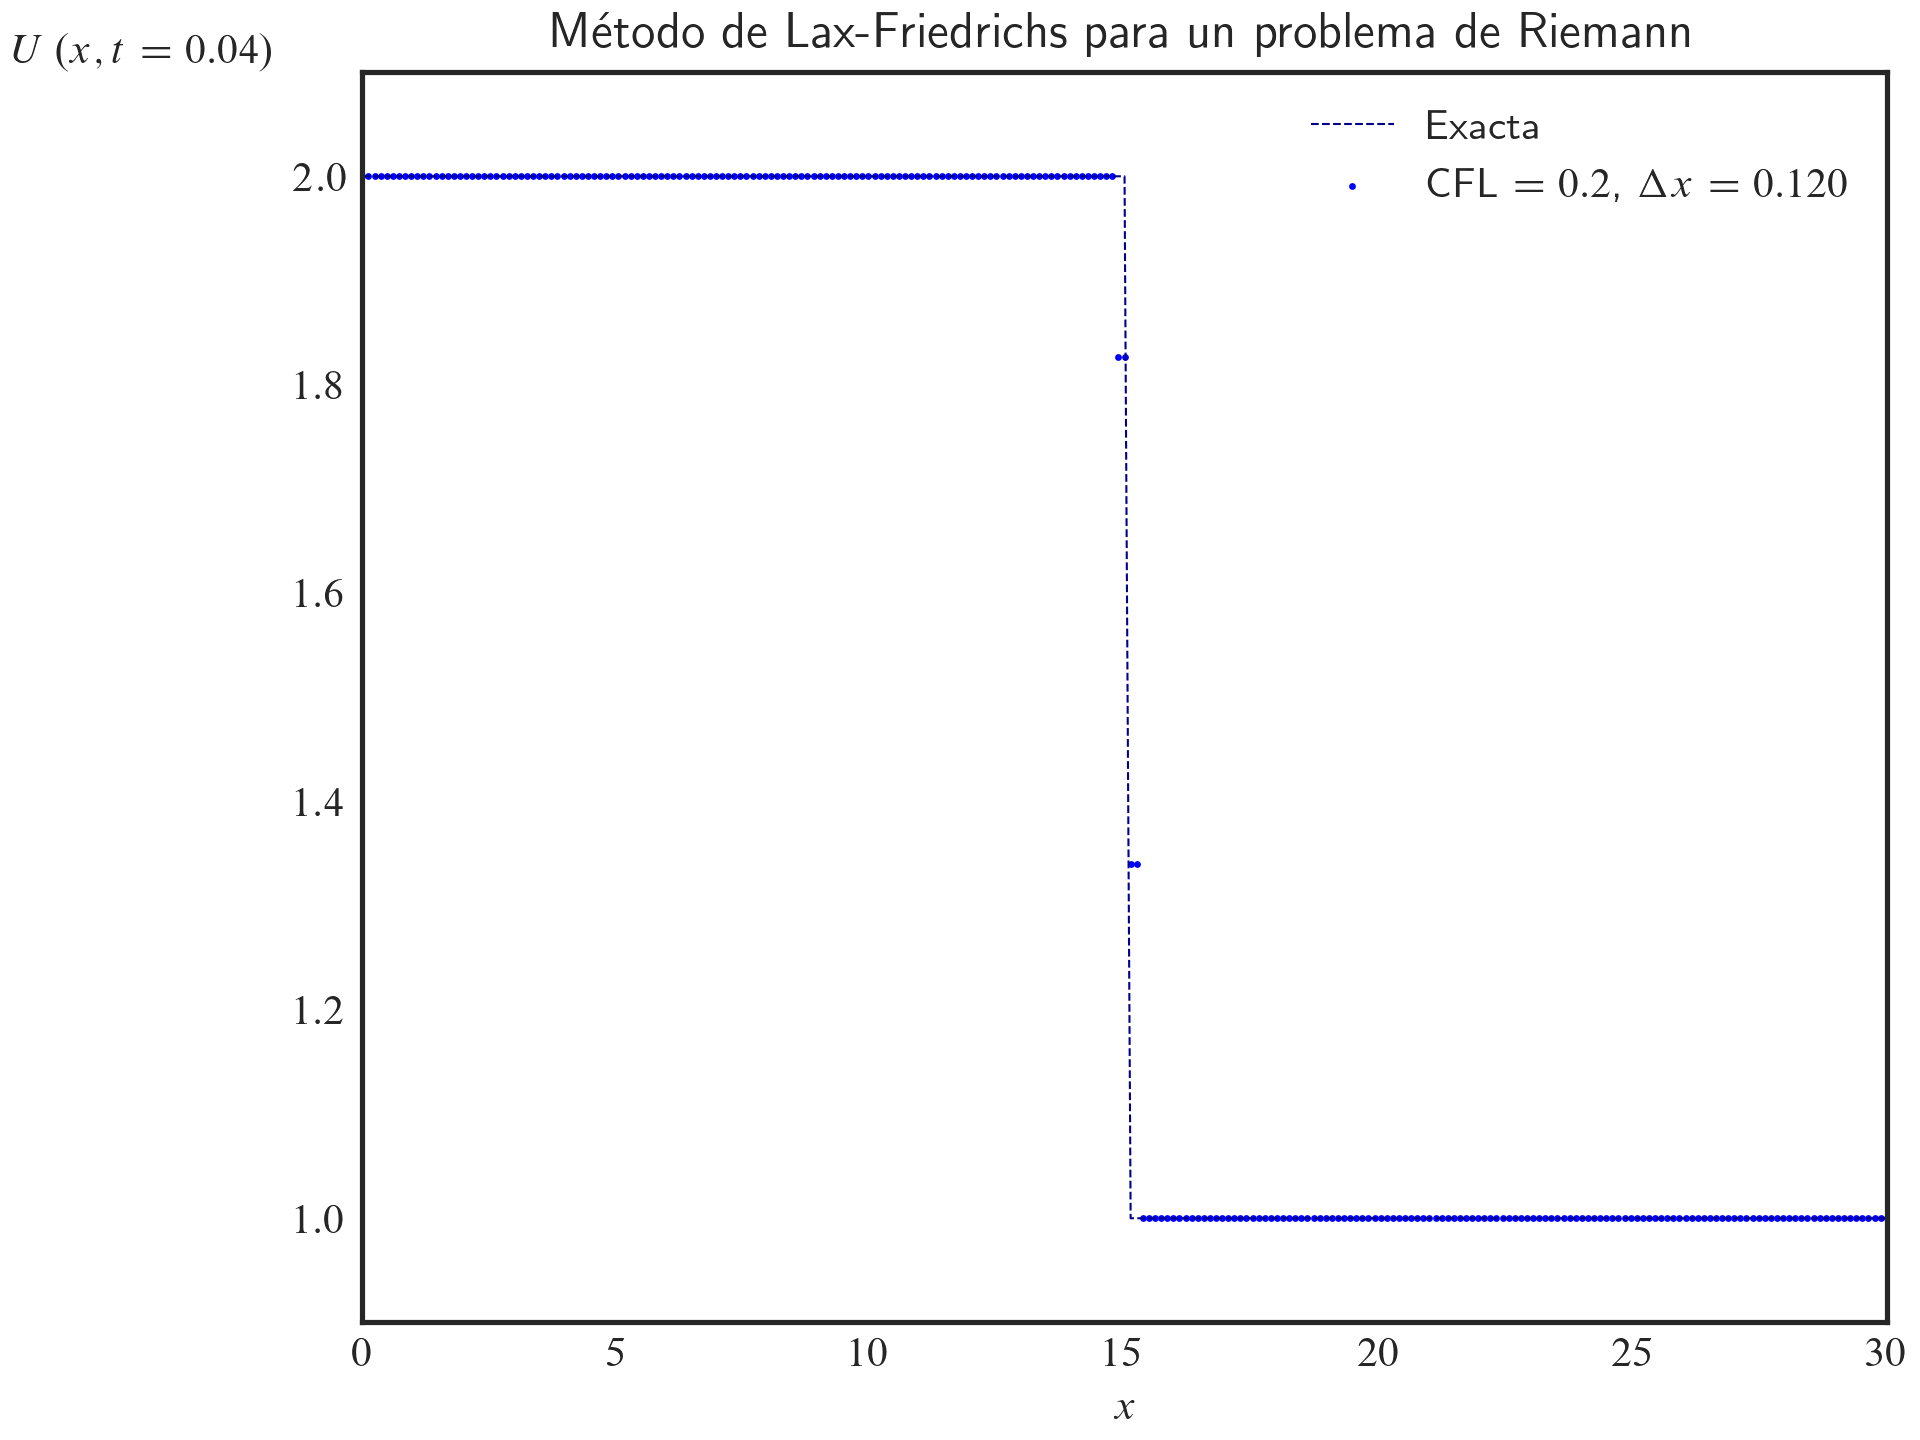
\includegraphics[width=.30\paperwidth]{../snapshots/lax-friedrichsheaviside1d-2.png}
        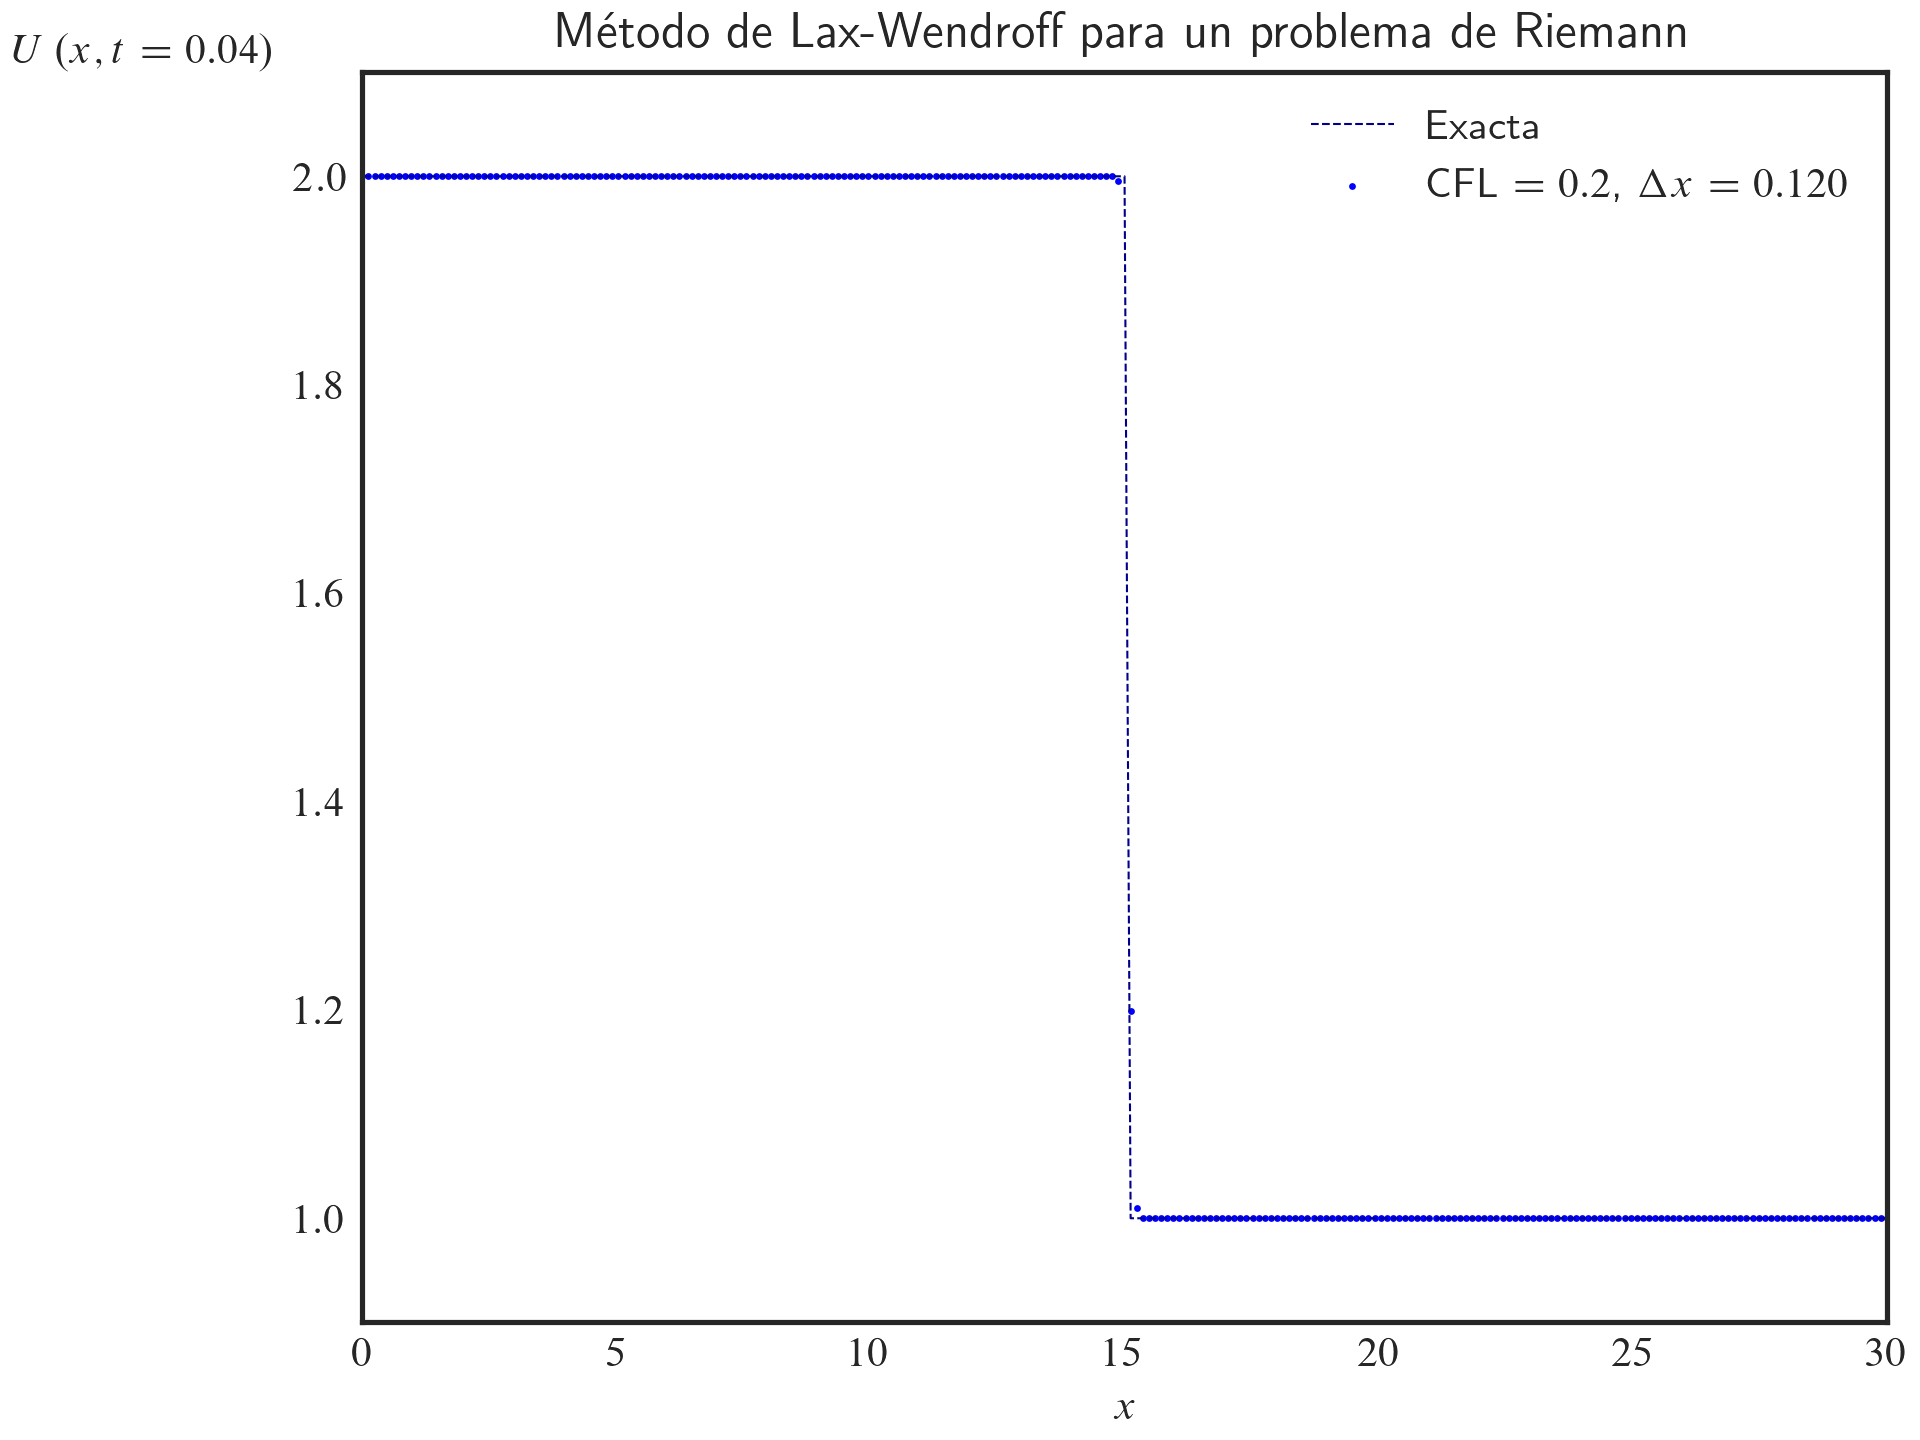
\includegraphics[width=.30\paperwidth]{../snapshots/lax-wendroffheaviside1d-2.png}
        \caption{Simulación numérica en el tiempo $t_{2}=2\Delta t$.}
        \label{fig:example2t2}
    \end{figure}

\end{frame}

\begin{frame}
    \frametitle{\secname}

    \begin{figure}[ht!]
        \centering
        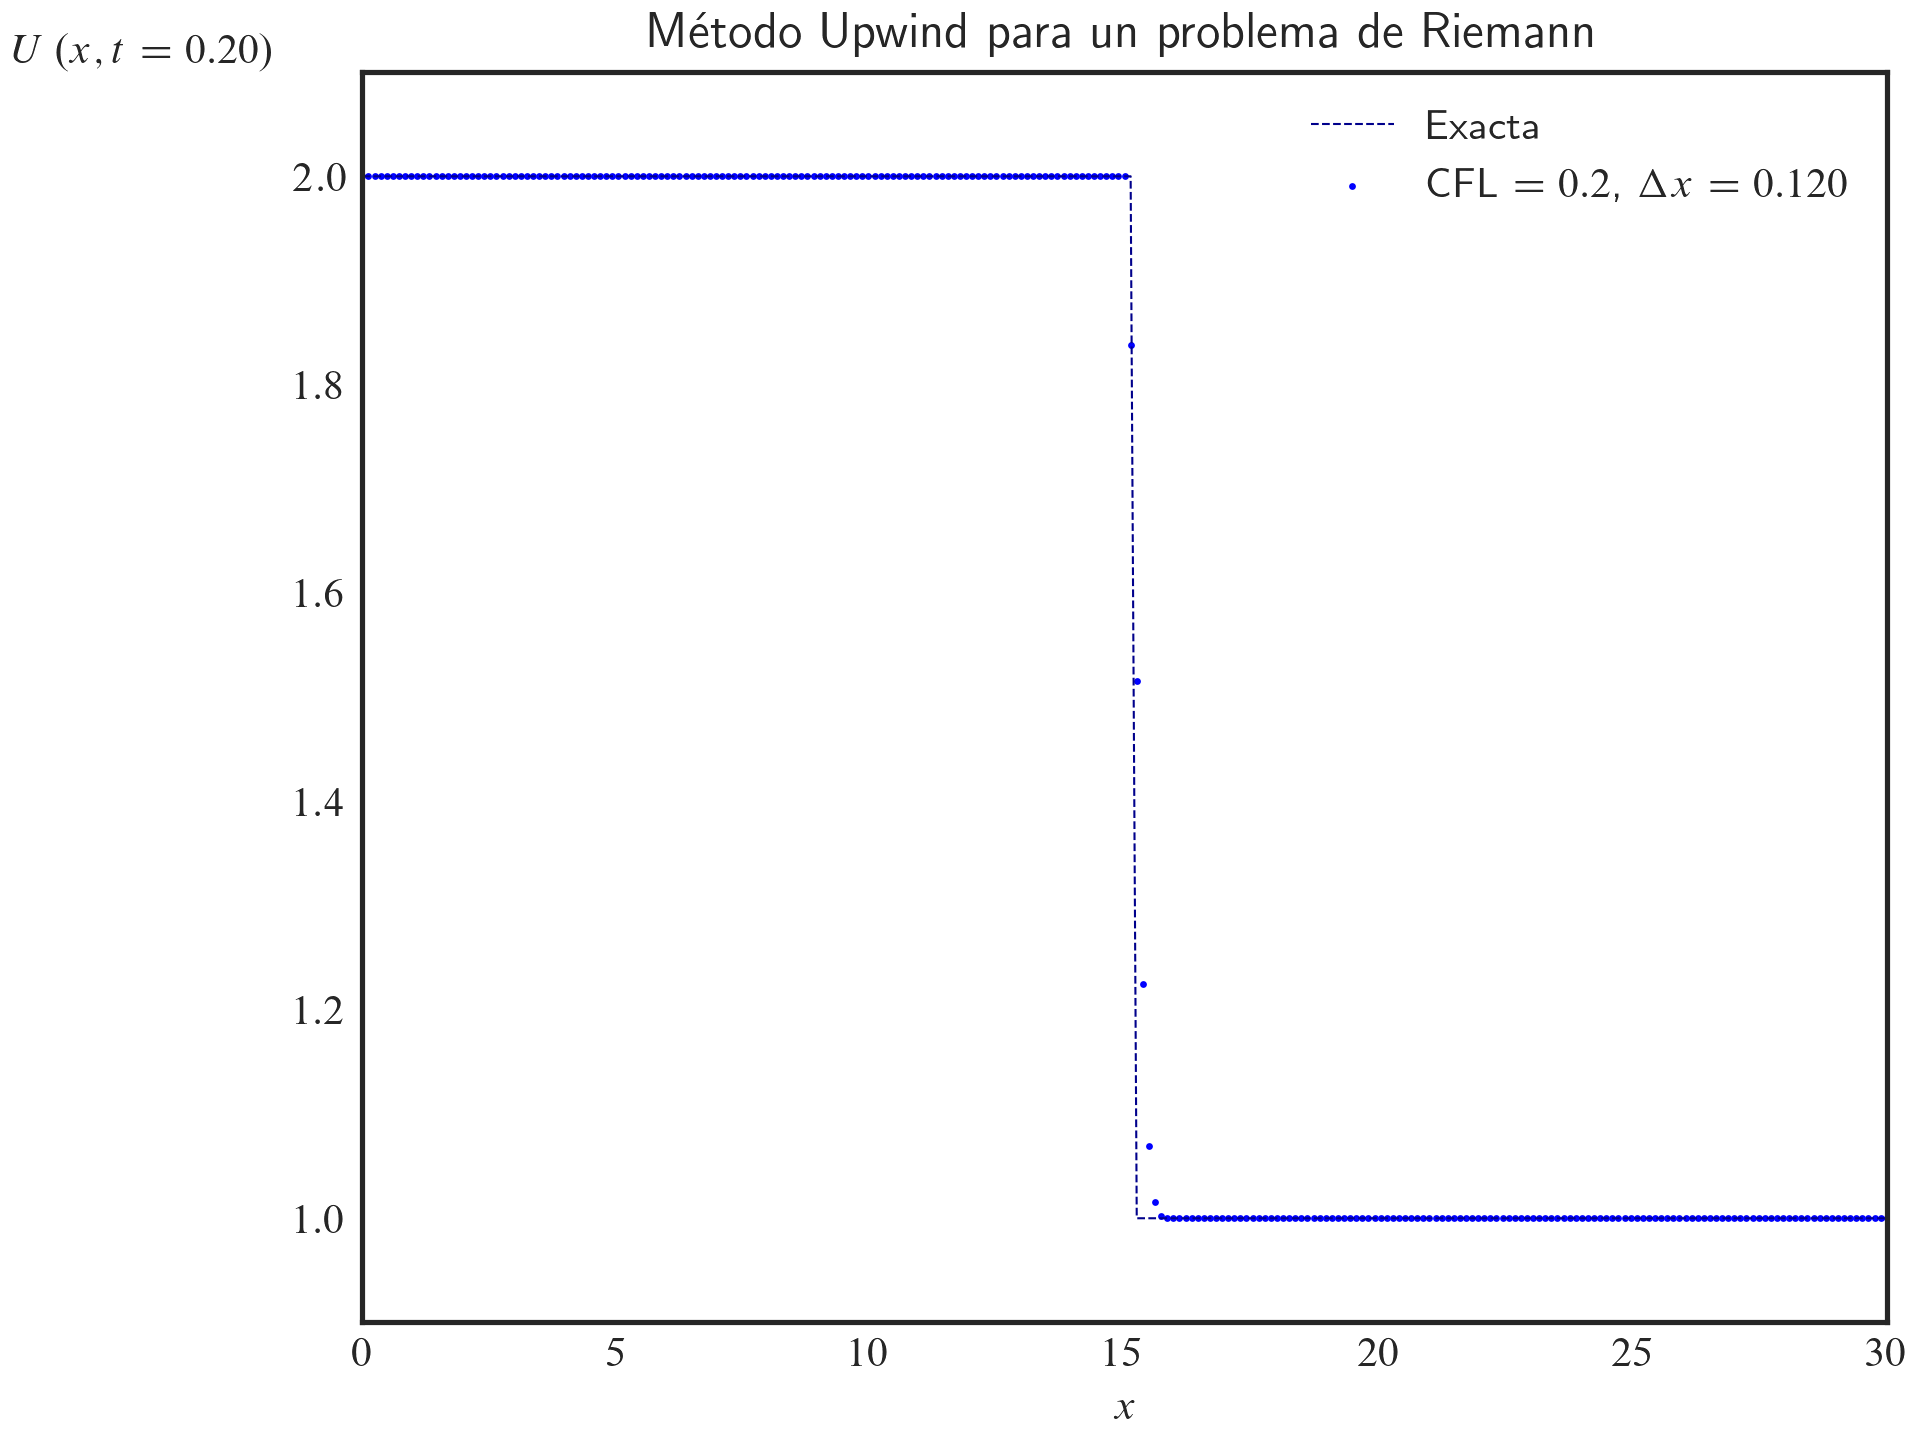
\includegraphics[width=.30\paperwidth]{../snapshots/upwindheaviside1d-10.png}
        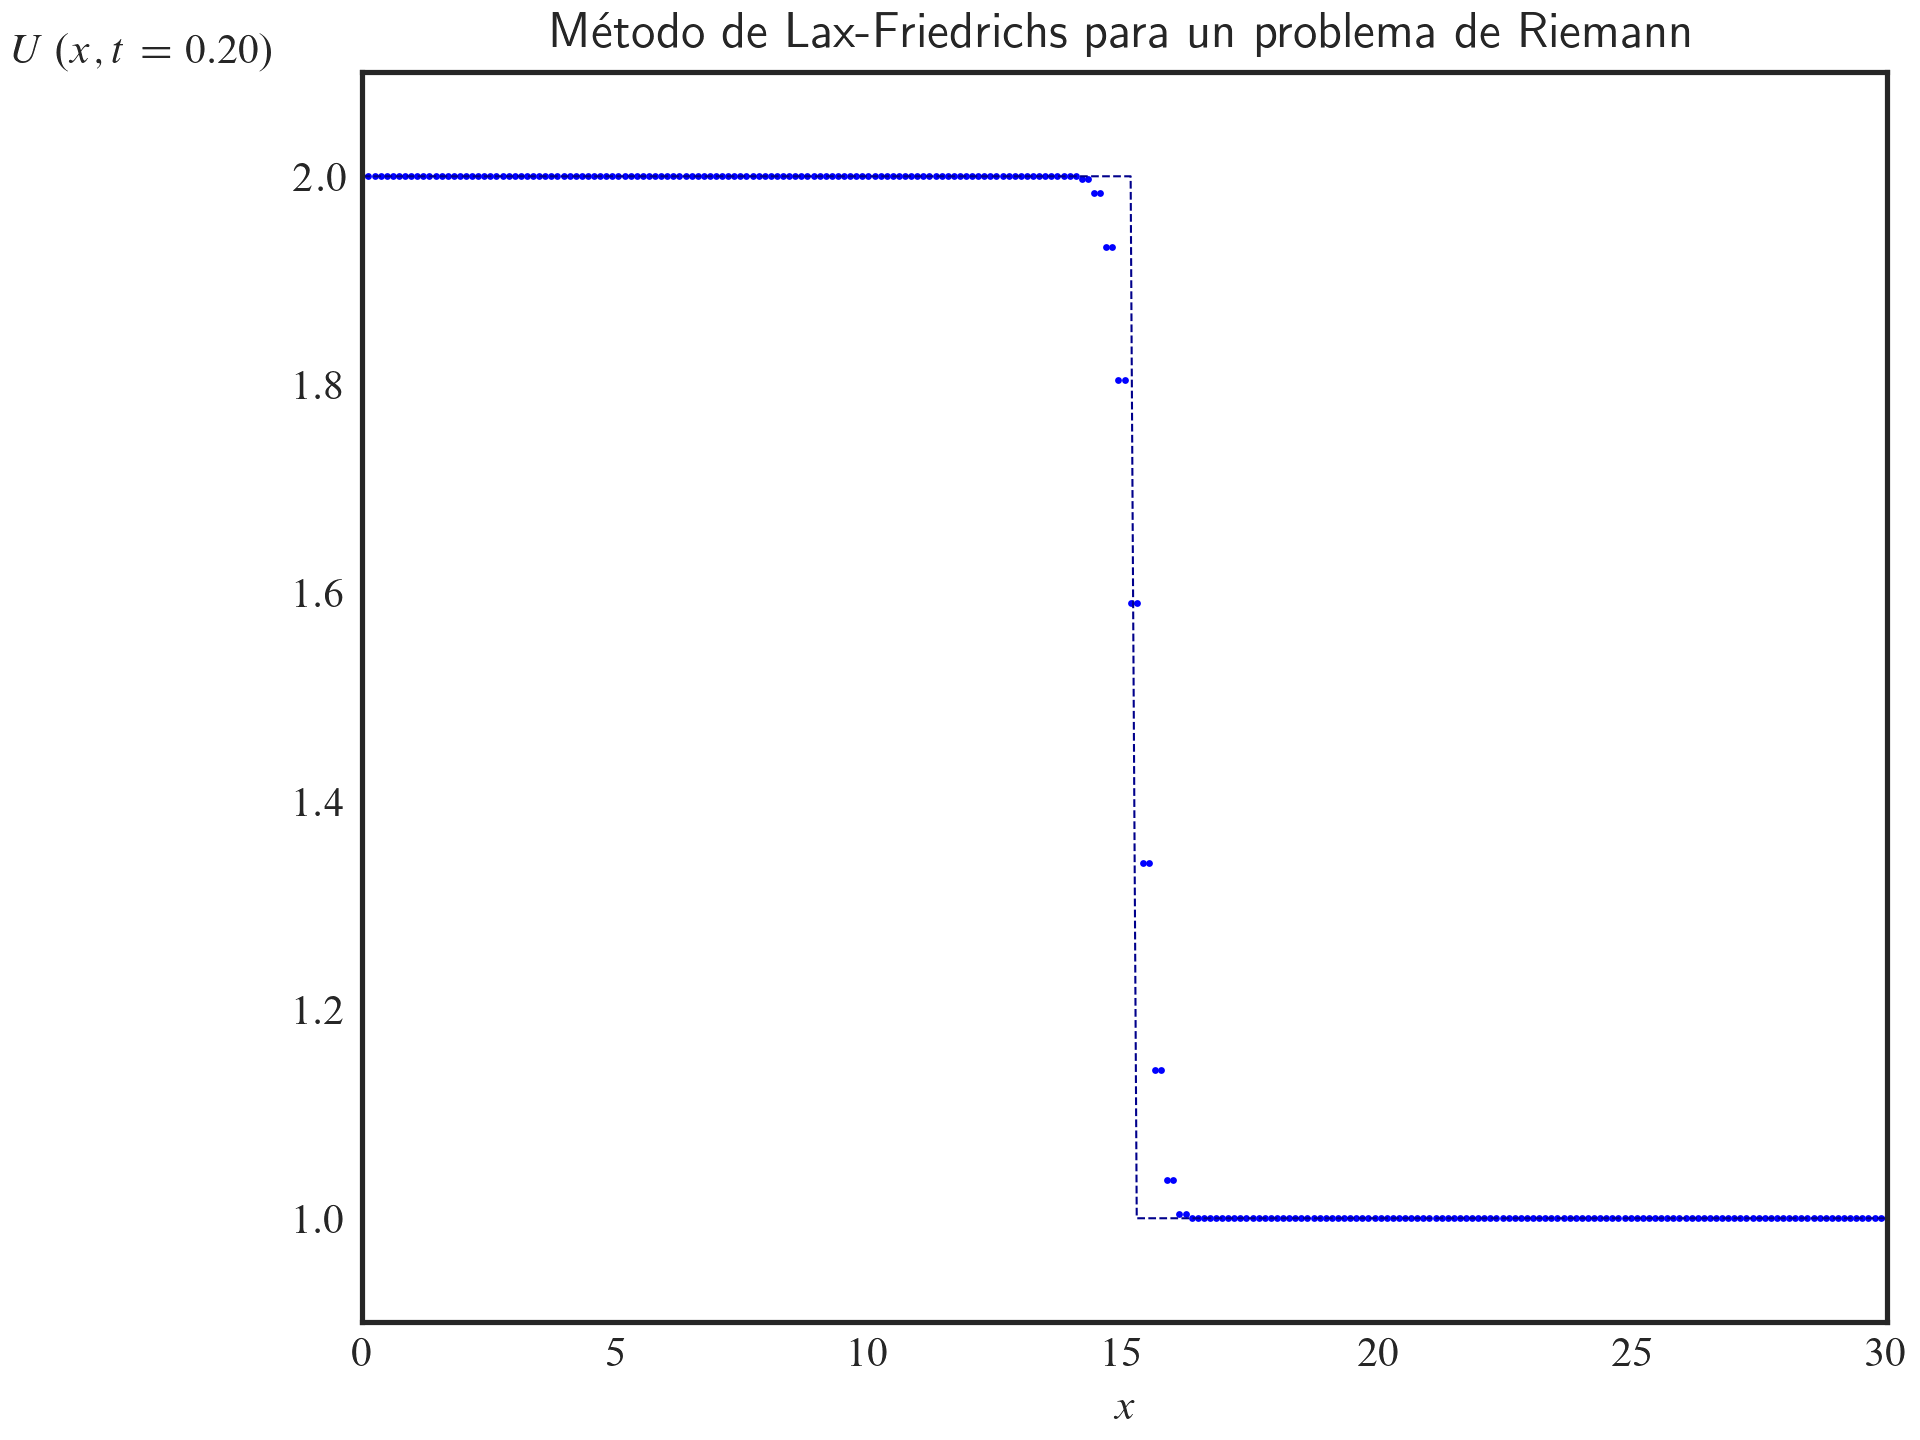
\includegraphics[width=.30\paperwidth]{../snapshots/lax-friedrichsheaviside1d-10.png}
        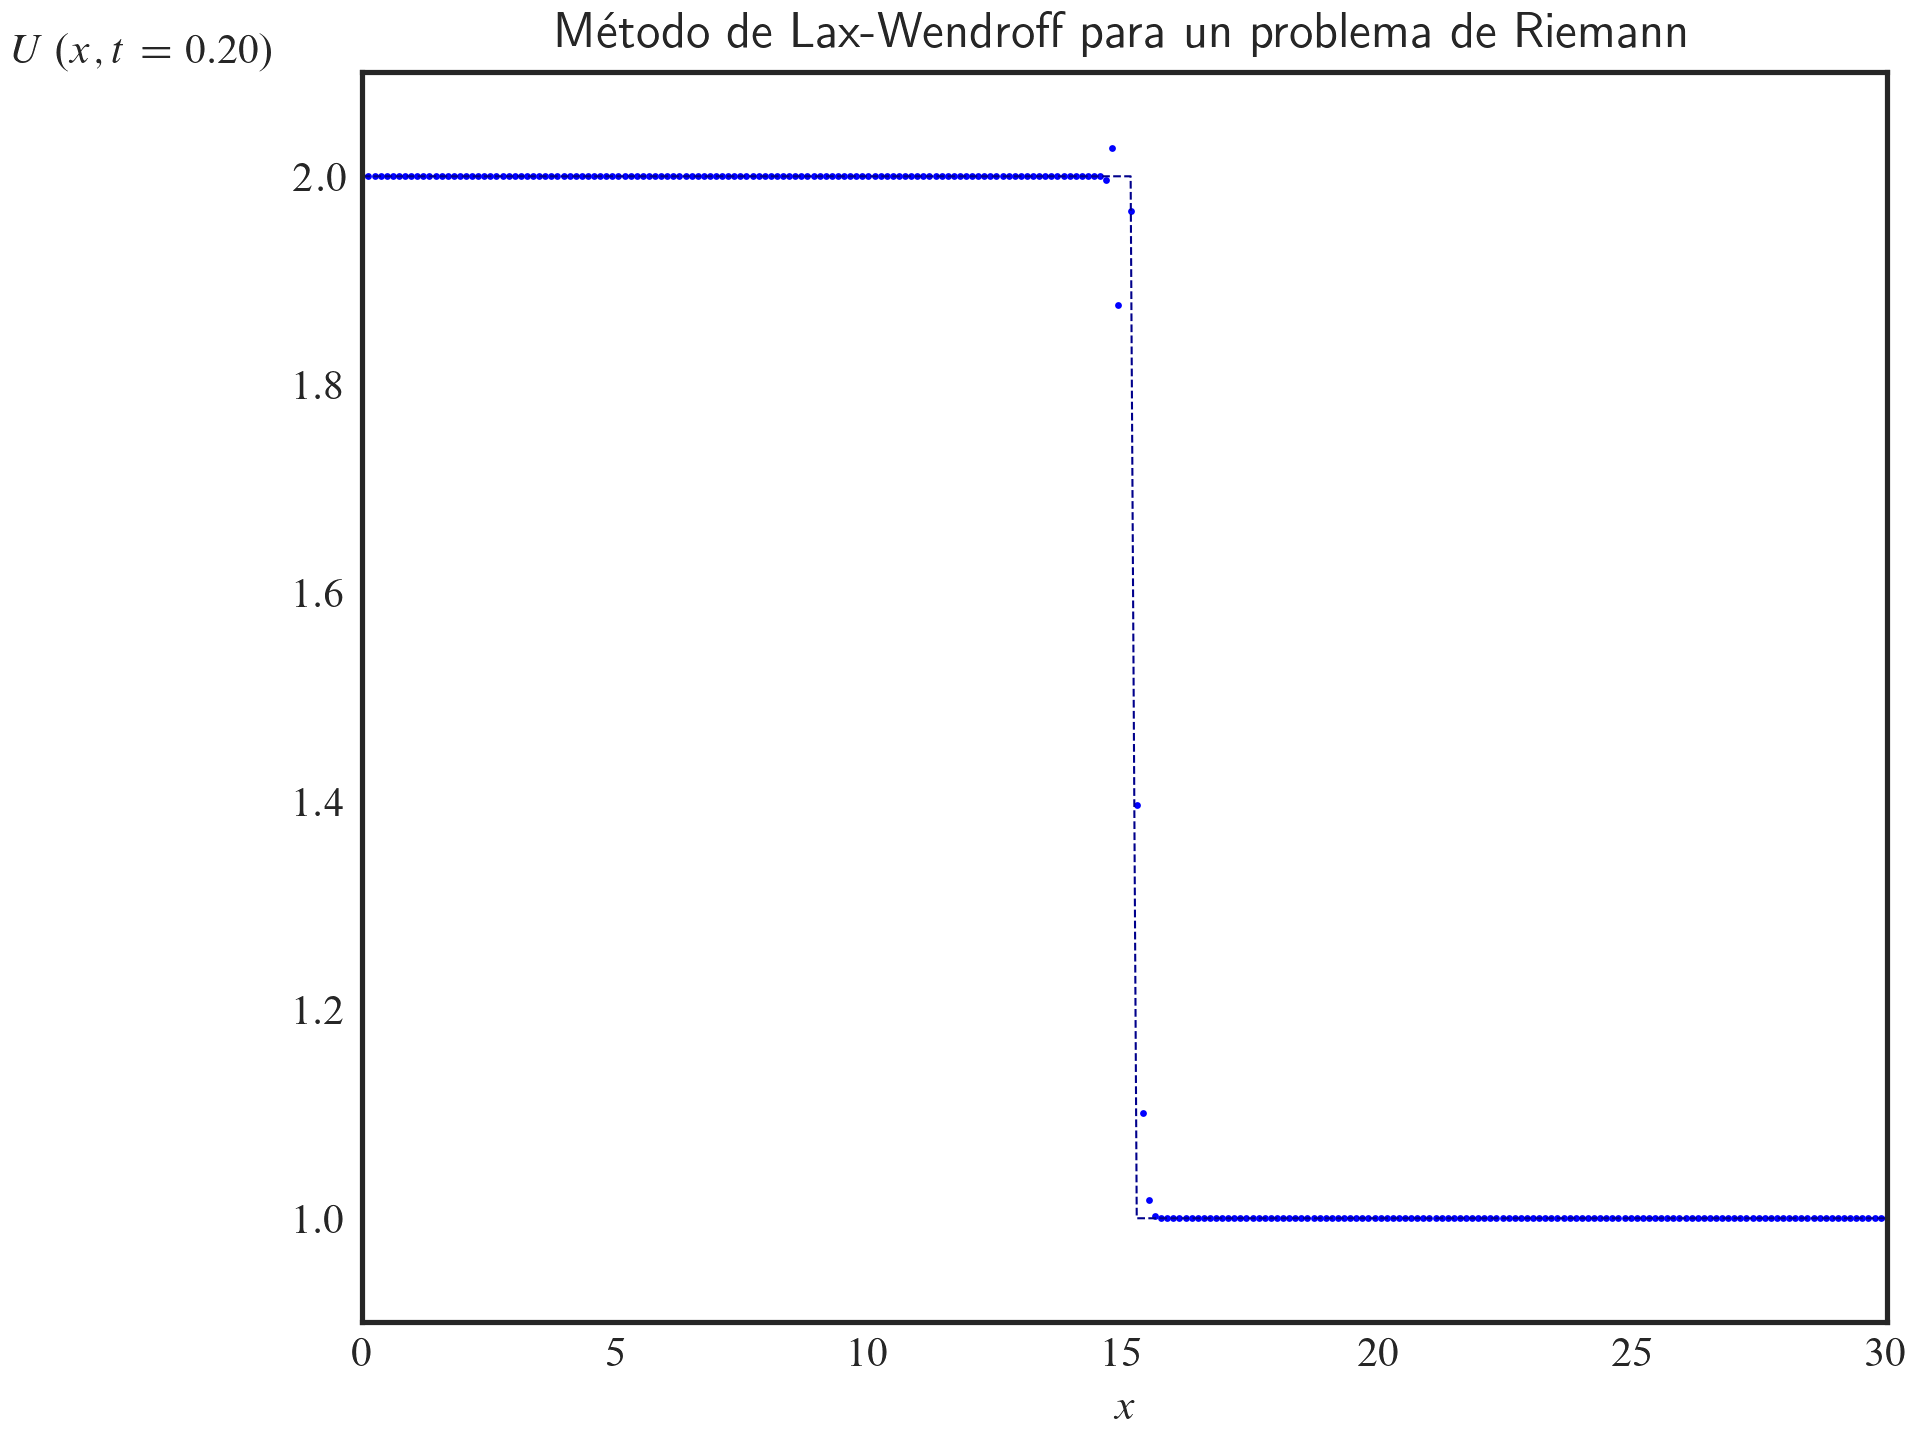
\includegraphics[width=.30\paperwidth]{../snapshots/lax-wendroffheaviside1d-10.png}
        \caption{Simulación numérica en el tiempo $t_{10}=10\Delta t$.}
        \label{fig:example2t10}
    \end{figure}
\end{frame}